%%%%%%%%%%%%%%%%%%%%%%%%%%%%%%%%%%%%%%%%%%%%%%%%%%%%%%%%%%
\frame {\frametitle{Setting up a Hadoop Cluster}
%%%%%%%%%%%%%%%%%%%%%%%%%%%%%%%%%%%%%%%%%%%%%%%%%%%%%%%%%%
  \begin{itemize}
  \item \textbf{Cluster deployment}
    \begin{itemize}
    \item Private cluster
    \item Cloud-based cluster
    \item AWS Elastic MapReduce
    \end{itemize}
    
    \vspace{20pt}
    
  \item \textbf{Outlook:}
    \begin{itemize}
    \item Cluster specification
      \begin{itemize}
      \item Hardware
      \item Network Topology
      \end{itemize}
    \item Hadoop Configuration
      \begin{itemize}
      \item Memory considerations
      \end{itemize}
    \end{itemize}  
  \end{itemize}  
}

%%%%%%%%%%%%%%%%%%%%%%%%%%%%%%%%%%%%%%%%%%%%%%%%%%%%%%%%%%
%%%%%%%%%%%%%%%%%%%%%%%%%%%%%%%%%%%%%%%%%%%%%%%%%%%%%%%%%%
\subsection{Specification}
%%%%%%%%%%%%%%%%%%%%%%%%%%%%%%%%%%%%%%%%%%%%%%%%%%%%%%%%%%
%%%%%%%%%%%%%%%%%%%%%%%%%%%%%%%%%%%%%%%%%%%%%%%%%%%%%%%%%%


%%%%%%%%%%%%%%%%%%%%%%%%%%%%%%%%%%%%%%%%%%%%%%%%%%%%%%%%%%
\frame {\frametitle{Cluster Specification}
%%%%%%%%%%%%%%%%%%%%%%%%%%%%%%%%%%%%%%%%%%%%%%%%%%%%%%%%%%
  \begin{itemize}
  \item \textbf{Commodity Hardware}
    \begin{itemize}
    \item Commodity $\neq$ Low-end
      \begin{itemize}
      \item False economy due to failure rate and maintenance costs
      \end{itemize}
    \item Commodity $\neq$ High-end
      \begin{itemize}
      \item High-end machines perform better, which would imply a
        smaller cluster
      \item A single machine failure would compromise a large fraction
        of the cluster
      \end{itemize}
    \end{itemize}

    \vspace{20pt}

  \item \textbf{A 2012 specification}:
    \begin{itemize}
    \item Dual socket, Two exacore
    \item 128 GB {\color{red}ECC} RAM
    \item 8 $\times$ 1 TB disks\footnote{\color{red}Why not using
        RAID instead of JBOD?}
    \item \{1,10\} Gigabit Ethernet
    \end{itemize}
  \end{itemize}
 
}

%%%%%%%%%%%%%%%%%%%%%%%%%%%%%%%%%%%%%%%%%%%%%%%%%%%%%%%%%%
\frame {\frametitle{Cluster Specification}
%%%%%%%%%%%%%%%%%%%%%%%%%%%%%%%%%%%%%%%%%%%%%%%%%%%%%%%%%%
  \begin{itemize}
  \item \textbf{Example:}
    \begin{itemize}
    \item Assume your data grows by 1 TB per week
    \item Assume you have three-way replication in HDFS
    \item[$\to$] You need additional 3TB of raw storage per week
    \item Allow for some overhead (temporary files, logs)
    \item[$\to$] {\color{red}This is a new machine per week}
    \end{itemize}

    \vspace{20pt}

  \item \textbf{How to dimension a cluster?}
    \begin{itemize}
    \item Obviously, you won't buy a machine per week!!
    \item The idea is that the above back-of-the-envelope calculation
      is that you can project over a 2 year life-time of your system
    \item[$\to$] You would need a 100-machine cluster 
    \end{itemize}

    \vspace{20pt}

  \item \textbf{Where should you put the various components?}
    \begin{itemize}
    \item Small cluster: NameNode and JobTracker can be
      {\color{red}collocated}
    \item Large cluster: requires more RAM at the NameNode
    \end{itemize}

  \end{itemize}
}

%%%%%%%%%%%%%%%%%%%%%%%%%%%%%%%%%%%%%%%%%%%%%%%%%%%%%%%%%%
\frame {\frametitle{Cluster Specification}
%%%%%%%%%%%%%%%%%%%%%%%%%%%%%%%%%%%%%%%%%%%%%%%%%%%%%%%%%%
  \begin{itemize}
  \item \textbf{Should we use 64-bit or 32-bit machines?}
    \begin{itemize}
    \item NameNode should run on a 64-bit machine: this avoids the
      3GB Java heap size limit on 32-bit machines
    \end{itemize}

    \vspace{40pt}

  \item \textbf{What's the role of Java?}
    \begin{itemize}
    \item Recent releases (Java6) implement some optimization to
      eliminate large pointer overhead
    \item[$\to$] A cluster of 64-bit machines has no downside
    \end{itemize}
  \end{itemize}

}
%%%%%%%%%%%%%%%%%%%%%%%%%%%%%%%%%%%%%%%%%%%%%%%%%%%%%%%%%%
%%%%%%%%%%%%%%%%%%%%%%%%%%%%%%%%%%%%%%%%%%%%%%%%%%%%%%%%%%
\subsection{Network Topology}
%%%%%%%%%%%%%%%%%%%%%%%%%%%%%%%%%%%%%%%%%%%%%%%%%%%%%%%%%%
%%%%%%%%%%%%%%%%%%%%%%%%%%%%%%%%%%%%%%%%%%%%%%%%%%%%%%%%%%

%%%%%%%%%%%%%%%%%%%%%%%%%%%%%%%%%%%%%%%%%%%%%%%%%%%%%%%%%%
\frame {\frametitle{Network Topology}
%%%%%%%%%%%%%%%%%%%%%%%%%%%%%%%%%%%%%%%%%%%%%%%%%%%%%%%%%%
   \begin{center}
      \framebox{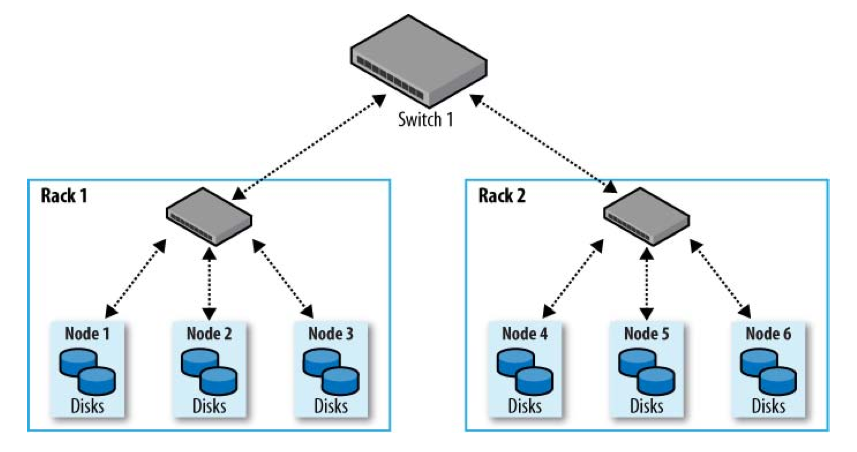
\includegraphics[scale=0.3]{./Figures/cluster_net_topology}}      
    \end{center}
}

%%%%%%%%%%%%%%%%%%%%%%%%%%%%%%%%%%%%%%%%%%%%%%%%%%%%%%%%%%
\frame {\frametitle{Network Topology}
%%%%%%%%%%%%%%%%%%%%%%%%%%%%%%%%%%%%%%%%%%%%%%%%%%%%%%%%%%
  \begin{itemize}
  \item \textbf{Two-level network topology}
    \begin{itemize}
    \item Switch redundancy is not shown in the figure
    \end{itemize}

\vspace{20pt}

  \item \textbf{Typical configuration}
    \begin{itemize}
    \item 30-40 servers per rack
    \item 10 GB switch TOR
    \item Core switch or router with 10GB or better
    \end{itemize}

\vspace{20pt}

  \item \textbf{Features}
    \begin{itemize}
    \item Aggregate bandwidth between nodes on the same rack is much
      larger than for nodes on different racks
    \item {\color{red}Rack awareness}
      \begin{itemize}
      \item Hadoop should know the cluster topology
      \item Benefits both HDFS (data placement) and MapReduce (locality)
      \end{itemize}
    \end{itemize}
  \end{itemize}
}

%%%%%%%%%%%%%%%%%%%%%%%%%%%%%%%%%%%%%%%%%%%%%%%%%%%%%%%%%%
%%%%%%%%%%%%%%%%%%%%%%%%%%%%%%%%%%%%%%%%%%%%%%%%%%%%%%%%%%
\subsection{Hadoop Configuration}
%%%%%%%%%%%%%%%%%%%%%%%%%%%%%%%%%%%%%%%%%%%%%%%%%%%%%%%%%%
%%%%%%%%%%%%%%%%%%%%%%%%%%%%%%%%%%%%%%%%%%%%%%%%%%%%%%%%%%

%%%%%%%%%%%%%%%%%%%%%%%%%%%%%%%%%%%%%%%%%%%%%%%%%%%%%%%%%%
\frame {\frametitle{Hadoop Configuration}
%%%%%%%%%%%%%%%%%%%%%%%%%%%%%%%%%%%%%%%%%%%%%%%%%%%%%%%%%%
  \begin{itemize}
  \item \textbf{There are a handful of files for controlling the operation of
      an Hadoop Cluster}
    \begin{itemize}
    \item Hundreds of parameters!!
    \item See next slide for a summary table
    \end{itemize}
    
    \vspace{20pt}
    
  \item \textbf{Managing the configuration across several machines}
    \begin{itemize}
    \item All machines of an Hadoop cluster must be in sync!
    \item What happens if you dispatch an update and some machines are
      down?
    \item What happens when you add (new) machines to your cluster?
    \item What if you need to patch MapReduce?
    \end{itemize}

    \vspace{20pt}
    
  \item \textbf{Common practice: use configuration management tools}
    \begin{itemize}
    \item Chef, Puppet, ...
    \item Declarative language to specify configurations
    \item Allow also to install software
    \end{itemize}
    
  \end{itemize}
}

%%%%%%%%%%%%%%%%%%%%%%%%%%%%%%%%%%%%%%%%%%%%%%%%%%%%%%%%%%
\frame {\frametitle{Hadoop Configuration}
%%%%%%%%%%%%%%%%%%%%%%%%%%%%%%%%%%%%%%%%%%%%%%%%%%%%%%%%%%
\begin{tiny}
  \begin{table}[h]
    \centering
    \begin{tabular}{||c|c|l||}
      \hline
      \hline
      {\textbf{Filename}} & {\textbf{Format}} & {\textbf{Description}} \\
      \hline
      \hline
      hadoop-env.sh & Bash script & {Environment variables that are
      used in the scripts to run Hadoop.} \\
      core-site.xml & Hadoop configuration XML & I/O settings that are common
      to HDFS and MapReduce.\\
      hdfs-site.xml  & Hadoop configuration XML & Namenode, the secondary
      namenode, and the datanodes. \\
      mapred-site.xml  & Hadoop configuration XML & Jobtracker, and the
      tasktrackers.\\
      masters & Plain text & A list of machines that
      each run a secondary namenode.\\
      slaves & Plain text & A list of machines that
      each run a datanode and a tasktracker. \\
      \hline
      \hline
    \end{tabular}
    \caption{Hadoop Configuration Files}
    \label{tab:conf}
  \end{table}
\end{tiny}
}

%%%%%%%%%%%%%%%%%%%%%%%%%%%%%%%%%%%%%%%%%%%%%%%%%%%%%%%%%%
\frame {\frametitle{Hadoop Configuration: memory utilization}
%%%%%%%%%%%%%%%%%%%%%%%%%%%%%%%%%%%%%%%%%%%%%%%%%%%%%%%%%%
  \begin{itemize}
  \item \textbf{Hadoop uses a lot of memory}
    \begin{itemize}
    \item Default values, for a typical cluster configuration
      \begin{itemize}
      \item DataNode: 1 GB
      \item TaskTracker: 1 GB
      \item Child JVM map task: 2 $\times$ 200MB
      \item Child JVM reduce task: 2 $\times$ 200MB
      \end{itemize}
    \end{itemize}

    \vspace{20pt}

  \item \textbf{All the moving parts of Hadoop (HDFS and MapReduce) can be
    individually configured}
    \begin{itemize}
    \item This is true for cluster configuration but also for {\color{red}job
      specific} configurations
    \end{itemize}

    \vspace{20pt}

  \item \textbf{Hadoop is fast when using RAM}
    \begin{itemize}
    \item Generally, MapReduce Jobs {\color{red}are not} CPU-bound
    \item Avoid I/O on disk as much as you can
    \item Minimize network traffic
      \begin{itemize}
      \item Customize the partitioner
      \item Use compression ($\to$ decompression is in RAM)
      \end{itemize}
    \end{itemize}
    
  \end{itemize}
}


%%%%%%%%%%%%%%%%%%%%%%%%%%%%%%%%%%%%%%%%%%%%%%%%%%%%%%%%%%
%%%%%%%%%%%%%%%%%%%%%%%%%%%%%%%%%%%%%%%%%%%%%%%%%%%%%%%%%%
\subsection{Cloud Deployments}
%%%%%%%%%%%%%%%%%%%%%%%%%%%%%%%%%%%%%%%%%%%%%%%%%%%%%%%%%%
%%%%%%%%%%%%%%%%%%%%%%%%%%%%%%%%%%%%%%%%%%%%%%%%%%%%%%%%%%

%%%%%%%%%%%%%%%%%%%%%%%%%%%%%%%%%%%%%%%%%%%%%%%%%%%%%%%%%%
\frame {\frametitle{Elephants in the cloud!}
%%%%%%%%%%%%%%%%%%%%%%%%%%%%%%%%%%%%%%%%%%%%%%%%%%%%%%%%%%
  \begin{itemize}
  \item \textbf{May organization run Hadoop in private clusters}
    \begin{itemize}
    \item Pros and cons
    \end{itemize}

\vspace{40pt}

  \item \textbf{Cloud based Hadoop installations (Amazon biased)}
    \begin{itemize}
    \item Use Cloudera + \{Whirr, boto, ...\}
    \item Use Elastic MapReduce
    \end{itemize}
  \end{itemize}
}

%%%%%%%%%%%%%%%%%%%%%%%%%%%%%%%%%%%%%%%%%%%%%%%%%%%%%%%%%%
\frame {\frametitle{Hadoop on EC2}
%%%%%%%%%%%%%%%%%%%%%%%%%%%%%%%%%%%%%%%%%%%%%%%%%%%%%%%%%%
  \begin{itemize}
  \item \textbf{Launch instances of a cluster on demand, paying by hour}
    \begin{itemize}
    \item CPU, in general bandwidth is used from within a datacenter,
      hence it's free
    \end{itemize}

    \vspace{20pt}

  \item \textbf{Apache Whirr project}
    \begin{itemize}
    \item Launch, terminate, modify a running cluster
    \item Requires AWS credentials
    \end{itemize}

    \vspace{20pt}

  \item \textbf{Example}
    \begin{itemize}
    \item Launch a cluster \texttt{test-hadoop-cluster}, with one
      master node (\texttt{JobTracker} and \texttt{NameNode}) and 5
      worker nodes (\texttt{DataNodes} and \texttt{TaskTrackers})
    \item[$\to$] \texttt{hadoop-ec2 launch-cluster test-hadoop-cluster
        5}
    \item See Chapter 9 \cite{hadoop_book}
    \end{itemize}
  \end{itemize}
}

%%%%%%%%%%%%%%%%%%%%%%%%%%%%%%%%%%%%%%%%%%%%%%%%%%%%%%%%%%
\frame {\frametitle{AWS Elastic MapReduce}
%%%%%%%%%%%%%%%%%%%%%%%%%%%%%%%%%%%%%%%%%%%%%%%%%%%%%%%%%%
  \begin{itemize}
  \item \textbf{Hadoop as a service}
    \begin{itemize}
    \item Amazon handles everything, which becomes transparent
    \item How this is done remains a mystery
    \end{itemize}

    \vspace{40pt}

  \item \textbf{Focus on What not How}
    \begin{itemize}
    \item All you need to do is to package a MapReduce Job in a JAR
      and upload it using a Web Interface
    \item Other Jobs are available: python, pig, hive, ...
    \item {\color{red}Test your jobs locally!!!}
    \end{itemize}
  \end{itemize}

}
